% coding:utf-8

%----------------------------------------
%FOSAPHY, a LaTeX-Code for a summary of basic physics
%Copyright (C) 2013, Mario Felder

%This program is free software; you can redistribute it and/or
%modify it under the terms of the GNU General Public License
%as published by the Free Software Foundation; either version 2
%of the License, or (at your option) any later version.

%This program is distributed in the hope that it will be useful,
%but WITHOUT ANY WARRANTY; without even the implied warranty of
%MERCHANTABILITY or FITNESS FOR A PARTICULAR PURPOSE.  See the
%GNU General Public License for more details.
%----------------------------------------

\chapter{Rotation}
\section{\"Ubersicht}
\begin{tabular}{|lp{.15\linewidth}|lp{0.15\linewidth}|}
		\hline
		\multicolumn{2}{|l|}{ROTATION} 			& \multicolumn{2}{l|}{LINEARE BEWEGUNG}\\
		\hline
		\rowcolor{lgray}Trägheitsmoment & $[kg \cdot m^2]$										& Masse&\\
		\multicolumn{2}{|l|}{$I=\sum{r_i^2m_i=\int{r^2\mathrm{d}m}}$}  				& \multicolumn{2}{l|}{$m$}\\
		\hline
		\rowcolor{lgray}Drehmoment & $[N \cdot m]$															& Kraft & $[N]$\\
		\multicolumn{2}{|l|}{$M=I \cdot \alpha$}																& \multicolumn{2}{l|}{$F=m\cdot a$}\\
		\hline
		\rowcolor{lgray}Drehimpuls & $[\frac{kg \cdot m^2}{s}]$									& Impuls & $[N\cdot s]$\\
		\multicolumn{2}{|l|}{$L=I \cdot \omega$}										  					& \multicolumn{2}{l|}{$p=m\cdot v$}\\
		\hline
		\rowcolor{lgray}Newtonsches Gesetz & $[N \cdot m]$											& Newtonsches Gesetz &\\
		\multicolumn{2}{|l|}{$M=\frac{\mathrm{d}L}{\mathrm{d}t}$}							& \multicolumn{2}{l|}{$F=\frac{\mathrm{d}p}{\mathrm{d}t}$}\\
		\hline
		\rowcolor{lgray}Rotationsenergie & $[J]$																& Kinetische Energie &\\
		\multicolumn{2}{|l|}{$E_{rot}=\frac{1}{2}I\omega^2$}										& \multicolumn{2}{l|}{$E_{kin}=\frac{1}{2}mv^2$}\\
		\hline
		\rowcolor{lgray}Leistung & $[W]$																				& Leistung &\\
		\multicolumn{2}{|l|}{$P=\frac{\mathrm{d}E}{\mathrm{d}t}=M\cdot\omega$}	& \multicolumn{2}{l|}{$P=F\cdot v$}\\
		\hline
\end{tabular}

\section{Kreisbewegung}
Bogenlänge $s$:
\[\boxed{s=r \cdot \theta} \]\\
Geschwindigkeit tagnetial $v$:
\[\boxed{v=r \cdot \omega=r\cdot\frac{\mathrm{d}\theta}{\mathrm{d}t}} \]\\
Beschleunigung tangential $a_{tan}$:
\[\boxed{a_{tan}=r \cdot \alpha=r\cdot\frac{\mathrm{d}^2\theta}{\mathrm{d}^2t}} \]\\
Beschleunigung raidal $a_{rad}$:
\[\boxed{a_{rad}=\frac{v^2}{r}=\omega^2\cdot r } \]\\

\section{Trägheitsmoment}
Definition bzgl. fester Achse:
\[
	\boxed{
		I=m_1r_1^2+m_2r_2^2+m_3r_3^2+\ldots=\sum{r_i^2m_i}=\int{r^2\mathrm{d}m}
	}
\]
$[I]=kg\cdot m^2$\\
\newline
Fehlende Massen haben negatives Trägheitsmoment!\\
\newline
\begin{footnotesize}
	Scheibe mit Loch: $I_{tot}=I^*+I_{Loch}$\\
	$I^*\Rightarrow I$ der Scheibe ohne Loch\\
	$I_{Loch}\Rightarrow$ negatives Moment
\end{footnotesize}

\subsection{Parallel Axis Theorem:}
\[
	\boxed{
		I_P=I_{cm}+m\cdot h^2
	}
\]

\newpage
\subsection{Trägheitsmoment regelmässiger Körper}

\begin{table}[h!]
\centering
\begin{tabular}{m{2cm} c m{0.4\textwidth}}
Körper        & Achse        & $I$ \\
\hline
& & \\
Kreisring, dünn &
        \begin{minipage}{0.3\textwidth}
        \centering
        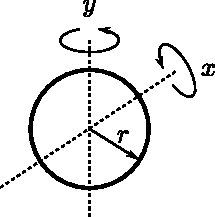
\includegraphics[scale=\traegscale]{../fig/traeg-kreisring-duenn.pdf}
        \end{minipage} &
                \begin{itemize}
                \item[$I_x$]$= m \cdot r^2$
                \item[$I_y$]$= \frac12 m\cdot r^2$
                \end{itemize} \\
Volltorus (Vollring) &
        \begin{minipage}{0.3\textwidth}
        \centering
        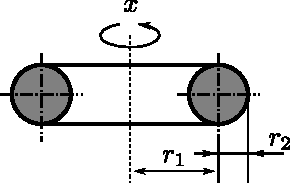
\includegraphics[scale=\traegscale]{../fig/traeg-kreisring.pdf}
        \end{minipage} &
                \begin{itemize}
                        \item[$I_x$]$= m \left({r_1}^2 + \frac{3}{4}
                                \cdot {r_2}^2\right)$
                \end{itemize} \\
Kreisbogen &
        \begin{minipage}{0.3\textwidth}
        \centering
        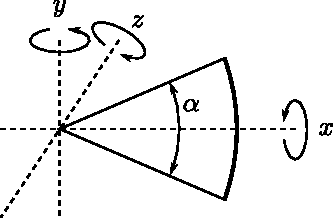
\includegraphics[scale=\traegscale]{../fig/traeg-kreisbogen.pdf}
        \end{minipage} &
                \begin{itemize}
                \item[$I_x$]$= \frac12 m \cdot r^2 
                        \left(1-\frac{sin(\alpha)}{\alpha} \right)$
                \item[$I_y$]$= \frac12 m \cdot r^2
                        \left(1+\frac{sin(\alpha)}{\alpha} \right)$
                \item[$I_z$]$= m \cdot r^2$
                \end{itemize} \\
Kreissektor &
        \begin{minipage}{0.3\textwidth}
        \centering
        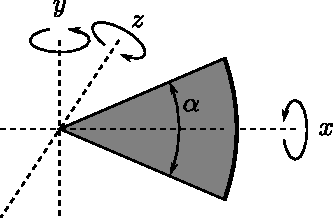
\includegraphics[scale=\traegscale]{../fig/traeg-kreissektor.pdf}
        \end{minipage} &
                \begin{itemize}
                \item[$I_x$]$= \frac14 m \cdot r^2
                        \left(1-\frac{sin(\alpha)}{\alpha} \right)$
                \item[$I_y$]$= \frac14 m \cdot r^2
                        \left(1+\frac{sin(\alpha)}{\alpha} \right)$
                \item[$I_z$]$= \frac12 m \cdot r^2$        
                \end{itemize} \\
Kreisscheibe, dünn &
        \begin{minipage}{0.3\textwidth}
        \centering
        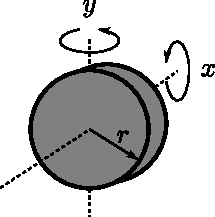
\includegraphics[scale=\traegscale]{../fig/traeg-kreisscheibe-duenn.pdf}
        \end{minipage} &
                \begin{itemize}
                \item[$I_x$]$= \frac12 m \cdot r^2$
                \item[$I_y$]$= \frac14 m \cdot r^2$
                \end{itemize} \\
Kugel, solid & \multirow{2}{*}{
        \begin{minipage}{0.3\textwidth}
        \centering
        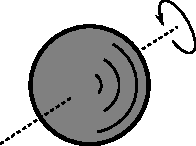
\includegraphics[scale=\traegscale]{../fig/traeg-kugel.pdf}
        \end{minipage}}
                &
                \begin{itemize}
                        \item[$I_x$]$= \frac{2}{5} m \cdot r^2$
                \end{itemize} \\
Kugel, dünnwandig & &
                \begin{itemize}
                        \item[$I_x$]$\approx \frac{2}{3} m \cdot r^2$
                \end{itemize}
\end{tabular}
\end{table}

\newpage
\begin{table}[h!]
\centering
\begin{tabular}{m{2cm} c m{0.4\textwidth}}
Körper        & Achse        & $I$ \\
\hline
& & \\
Stab &
        \begin{minipage}{0.3\textwidth}
        \centering
        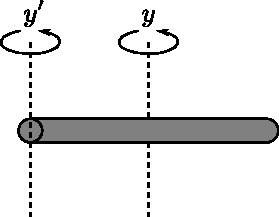
\includegraphics[scale=\traegscale]{../fig/traeg-stab.pdf}
        \end{minipage} &
                \begin{itemize}
                \item[$I_y$]$= \frac{1}{12} m \cdot l^2$
                \item[$I_{y'}$]$= \frac{1}{3} m \cdot l^2$
                \end{itemize} \\
& & \\
Vollzylinder &
        \begin{minipage}{0.3\textwidth}
        \centering
        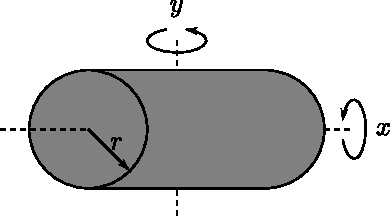
\includegraphics[scale=\traegscale]{../fig/traeg-vollzylinder.pdf}
        \end{minipage} &
                \begin{itemize}
                \item[$I_x$]$= \frac12 m \cdot r^2$
                \item[$I_y$]$= \frac{1}{12} m \left( 3r^2 + l^2 \right)$
                \end{itemize} \\
& & \\
Hohlzylinder, dünnwandig &
        \begin{minipage}{0.3\textwidth}
        \centering
        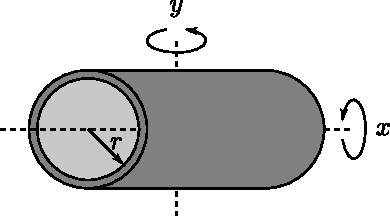
\includegraphics[scale=\traegscale]{../fig/traeg-hohlzylinder-duenn.pdf}
        \end{minipage} &
                \begin{itemize}
                \item[$I_x$]$= m \cdot  r^2$
                \item[$I_y$]$= \frac12 m (r^2 + \frac16 l^2)$
                \end{itemize} \\
& & \\
Hohlzylinder &
        \begin{minipage}{0.3\textwidth}
        \centering
        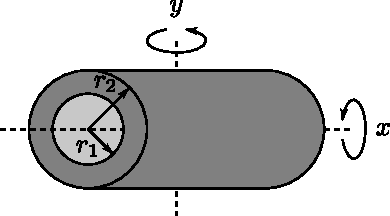
\includegraphics[scale=\traegscale]{../fig/traeg-hohlzylinder.pdf}
        \end{minipage} &
                \begin{itemize}
                \item[$I_x$]$= \frac12 m \left({r_1}^2 + {r_2}^2 \right)$
                \item[$I_y$]$= \frac14 m \left({r_1}^2 + {r_2}^2
                        + \frac13 l^2 \right)$
                \end{itemize}\\
Quader &
        \begin{minipage}{0.3\textwidth}
        \centering
        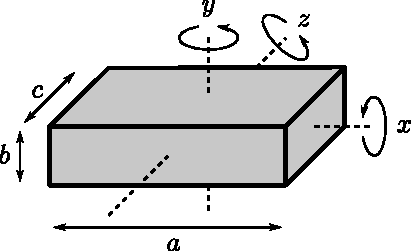
\includegraphics[scale=\traegscale]{../fig/traeg-quader.pdf}
        \end{minipage} &
                \begin{itemize}
                \item[$I_x$]$= \frac{1}{12} m \left(b^2 + c^2\right)$
                \item[$I_y$]$= \frac{1}{12} m \left(a^2 + c^2\right)$
                \item[$I_z$]$= \frac{1}{12} m \left(a^2 + b^2\right)$
                \end{itemize} \\
Platte, dünn &
        \begin{minipage}{0.3\textwidth}
        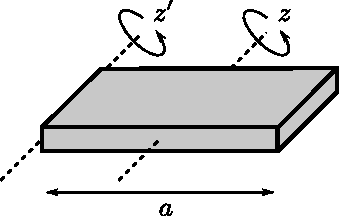
\includegraphics[scale=\traegscale]{../fig/traeg-platte.pdf}
        \end{minipage} &
                \begin{itemize}
                \item[$I_z$]$= \frac{1}{12} m \cdot a^2$
                \item[$I_{z'}$]$= \frac{1}{3} m \cdot a^2$
                \end{itemize} \\
\end{tabular}
\end{table}

\newpage

\section{Perfektes Rollen}
\[
	\boxed{
		v_{cm}=R\cdot \omega
	}
\]
\subsection{Momentane Drehachse P}
Beim perfekten Rollen ist der Kontaktpunkt P zwischen Rad und Unterlage momentan in Ruhe:
\[
	\boxed{
		E_{pot}=E_{kin,cm}+E_{rot,cm}=E_{rot,P}
	}
\]

\section{Drehmoment $\vec{M}$}
Definition:
\[
	\boxed{
		\vec{M}=\vec{r} \times \vec{F}
	}
\]
$[M]=Nm$\\
\newline
Das Drehmoment ist \textbf{senkrecht} zu $\vec{F}$ und $\vec{r}$.\\
\newline
Rotation eines starren Körpers um feste Achse:
\[
	\boxed{
		\sum{\vec{M}_i}=\vec{M}_{res} = I\vec{\alpha}
	}
\]\\
\newline
Teilchengeschwindigkeit:
\[
	\boxed{
		\vec{v}_i=\vec{v}_{cm}+\vec{v}_{i,rel}=\vec{v}_{cm}+\vec{\omega}\times\vec{r}_i
	}
\]

\section{Arbeit und Leistung (rot.)}
Bei der Rotation verrichtete \textbf{Arbeit}:
\[
	\boxed{
		W=\int_{\omega 1}^{\omega 2}{I\omega_z\mathrm{d}\omega_z}=\frac{1}{2}I\omega_2^2-\frac{1}{2}I\omega_1^2
	}
\]\\
\newline
Bei der Rotation verrichtete \textbf{Leistung}:
\[
	\boxed{
		P=M_z\omega_z
	}
\]

\section{Drehimpuls $\vec{L}$ und Drallsatz}
Definition:
\[
	\boxed{
		\vec{L}=\vec{r}\times\vec{p}=\vec{r}\times m\vec{v}
	}
\]\\
$[L]=\frac{kg\cdot m^2}{s}$\\
\newline
Drehimpuls für Symmetrieachse von starrem Körper:
\[
	\boxed{
		\vec{L}=I\cdot\vec{\omega}
	}
\]\\
\newline
Drallsatz (Newton für die Rotation):
\[
	\boxed{
		\sum{\vec{M}}=\frac{\mathrm{d}\vec{L}}{\mathrm{d}t}
	}
\]
\newpage
\section{Präzession}
Die Schwerkraft bewirkt das Drehmoment:
\[
	M=r\times mg
\]
Mit $r$ als Abstand des Schwerpunkts zum Unterstützungspunkt.\\
\newline
Da $M$ senkrecht zu $r$ und $F_g$ ist, ist es auch senkrecht zum Drehimpuls $L$. Daher ändert sich nur dessen Richtung, nicht jedoch der Betrag. Somit dreht sich der Kreisel horizontal. Es ist:
\[
	\begin{split}
		&\frac{\mathrm{d}L}{L}=\mathrm{d}\varphi\\
		\Rightarrow\ \ &M=\frac{\mathrm{d}L}{\mathrm{d}t}=L\frac{\mathrm{d}\varphi}{\mathrm{d}t}
	\end{split}
\]\\
Die Winkelgeschwindigkeit $\omega_P$ diser Rotation beträgt ($w_P\ll w_K$):
\[
	\boxed{
		\omega_P=\frac{\mathrm{d}\varphi}{\mathrm{d}t}=\frac{M}{L}=\frac{mgr}{I\omega_K}
	}
\]
\begin{footnotesize}
	$w_P$ auch als $\Omega$\\
\end{footnotesize} 

\begin{figure}[h!]
\center
\piccaption{Päzession\label{prazession}}
\parpic{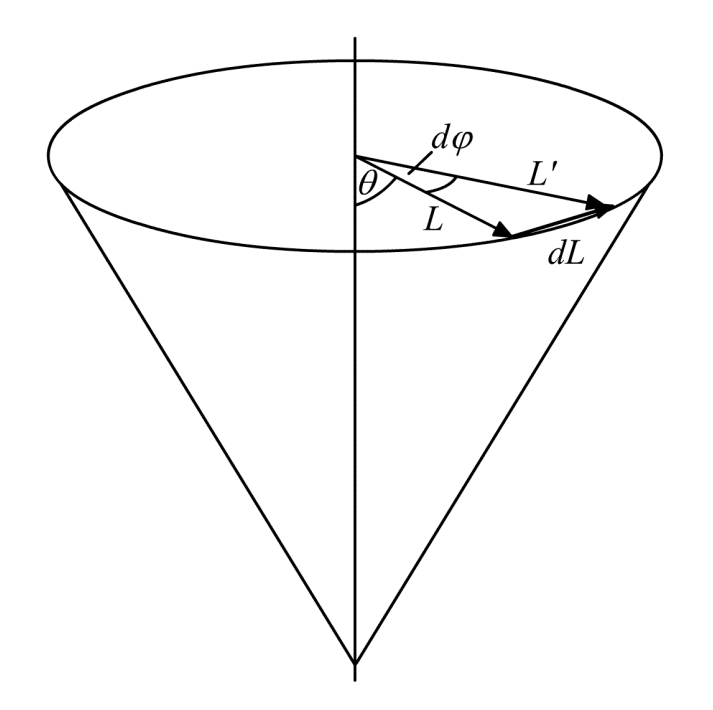
\includegraphics[scale=0.8]{../fig/prazession}}
\end{figure}
